\documentclass[12pt,letterpaper]{article}
\usepackage[spanish]{babel}
\usepackage[utf8]{inputenc}
\usepackage{fancyhdr}
\usepackage{amsmath}
\usepackage{amsfonts}
\usepackage{amssymb}
\usepackage{float}
\usepackage{graphicx}
\author{Irarrázabal Callejas Norton John\\Villalobos Gebre Gonzalo Andres\\Urrutia Torres Sebastián Felipe\\Valdivia Astudillo Juan Pablo\\Pérez Olivares Angelo Hernán\\Universidad de La Serena\\Facultad de Ciencias}
\title{Documentacion - Algoritmos de ordenamiento }
\date{}
\usepackage{listings}
\usepackage{multicol}
\usepackage[right=2cm,left=3cm,top=2cm,bottom=2cm,headsep=0cm,footskip=0.5cm]{geometry}
%-------------------------------------------------------------------------
\begin{document}
\maketitle
\begin{figure} [H]
\begin {center}
%\includegraphics[width=10cm,height=5cm]{imagenavl} 
\end {center}
\end{figure}
%-------------------------------------------------------------------------
\newpage
\tableofcontents
%-------------------------------------------------------------------------
\newpage
\section{Introducción}
\vskip 0.4cm
En la presente documentacion se abordaran los algoritmos de ordenamiento que nos permiten, reorganizar el orden de los elementos de una estructura, como por ejemplo un vector. En una secuencia definida por una relacion de orden (generalmente ascendentes o descendentes). Las relaciones de orden más usadas son el orden numérico y el orden lexicográfico. Los ordenamientos eficientes, son importantes para optimizar el uso de otros algoritmos como los de búsqueda que requieren listas ordenadas para una ejecución rápida.
 \vskip 0.4cm
Existen dos clases generales de técnicas de ordenamiento, Internas y Externas. La ordenación Interna se lleva a cabo en la memoria principal, lo que significa que es utilizada la memoria de acceso directo de alta velocidad, mientras que la ordenación Externa, hace uso del almacenamiento secundario que es más lento. Esta última técnica se usa en general para cuando se tiene una gran cantidad de datos, que hacen difícil el usar la memoria principal para guardarlos. El problema en este sentido es el movimiento de datos que se genera entre la unidad
externa de almacenamiento y la memoria principal. 
 \vskip 0.4cm
¿Los algoritmos son todos iguales? No, algunos son mas eficientes que otros, la eficiencia es determianda por el Orden de los algoritmos es decir el numero de operaciones que hay que hacer para ordenar una estrucutura de N elementos. generalmente el orden esta definido como:
 \vskip 0.4cm
\begin{itemize}
\item Orden lineal
\item Orden exponencial
\item Orden logaritmico
\end{itemize}

\vskip 0.4cm
Describiremos 3 algoritmos para ordenar la informacion: 
\vskip 0.4cm
\begin{itemize}
\item Insertion sort: Es un algoritmo basado en comparaciones eficiente para clasificar un numero pequeño de elementos. Este tipo de algoritmos funcionan identico a cuando las personas ordenan una mano de cartas. Requiere O($n^2$) operaciones para ordenar una lista de n elementos.
\end{itemize}
\vskip 0.4cm
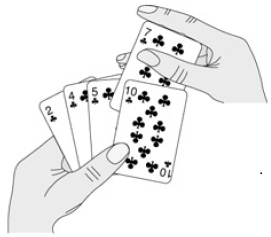
\includegraphics[width=8cm,height=7cm]{Imagen1}
\vskip 0.4cm
Enfoque dividir para conquistar: Este enfoque divide un problema en varios subproblemas que son similares al problema original pero de menor tamaño, resuelve los subproblemas recursivamente, y luego combina las soluciones, para crear la solucion al problema original.
\vskip 0.4cm
\begin{itemize}
\item Merge sort: El algoritmo de ordenamiento por mezcla (merge sort en inglés) es un algoritmo de ordenamiento externo estable basado en la técnica divide y vencerás. Es de complejidad O(n log n). Fue desarrollado en 1945 por John Von Neumann.
\vskip 0.4cm
Conceptualmente, funciona de la siguiente manera:

1. Divida la lista sin ordenar en n sublistas, cada una con 1 elemento (una lista de 1 elemento se considera ordenada).
\vskip 0.4cm
2. Repetidamente mezclar sublistas para producir nuevas sublistas ordenadas hasta que sólo quede 1 sublista. Esta será la lista ordenada.
\end{itemize}
\vskip 0.4cm
\begin{itemize}
\item Quick sort: Basado igualmente en la metodologia dividir para conquistar. Dado un array A de n-elementos trabaja de la siguiente forma: 
La ordenación rápida divide A en dos subarrays que pueden ser ordenados de forma independiente.
Se selecciona un elemento especifico del array A[p] llamado pivote, seguidamente se recorre el
array desde la izquierda hasta encontrar una llave mayor que el pivote, y desde la derecha hasta
encontrar una menor, una vez ocurrido se intercambian, el proceso se repite hasta que los índices de
incremento y decremento se cruzan. En esta situación notar que, el array está dividido en dos partes,
la izquierda con todos los elementos menores que el pivote y la derecha con todos los mayores. A
cada una de estas partes se le llama partición,  luego el método se repite para cada una de las
particiones y así sucesivamente hasta que no haya particiones a ordenar.
En el caso promedio, el orden es O(n·log n).
\end{itemize}
\vskip 0.4cm
Tambien se presentara el método Arrays.sort() de Java, este .sort () es un método de clase java.util.Arrays.
Donde la clase Arrays contiene varios metodos para la manipuacion de arreglos (ordenamiento y busqueda). Esta clase tambien permite que los arreglos se puedan ver como listas. Nosotros nos centraremos en los metodos sort para arreglos. Que nos sirve para ordenar ya sea de forma ascendente o descendente, Y tambien permite organizar una parte del arreglo a partir de un determinado indice.
\vskip 0.4cm
El metodo sort varia dependiendo de los parametros que se le incluyan en el llamado.
Como se muestra en la siguiente imagen:
\vskip 0.4cm
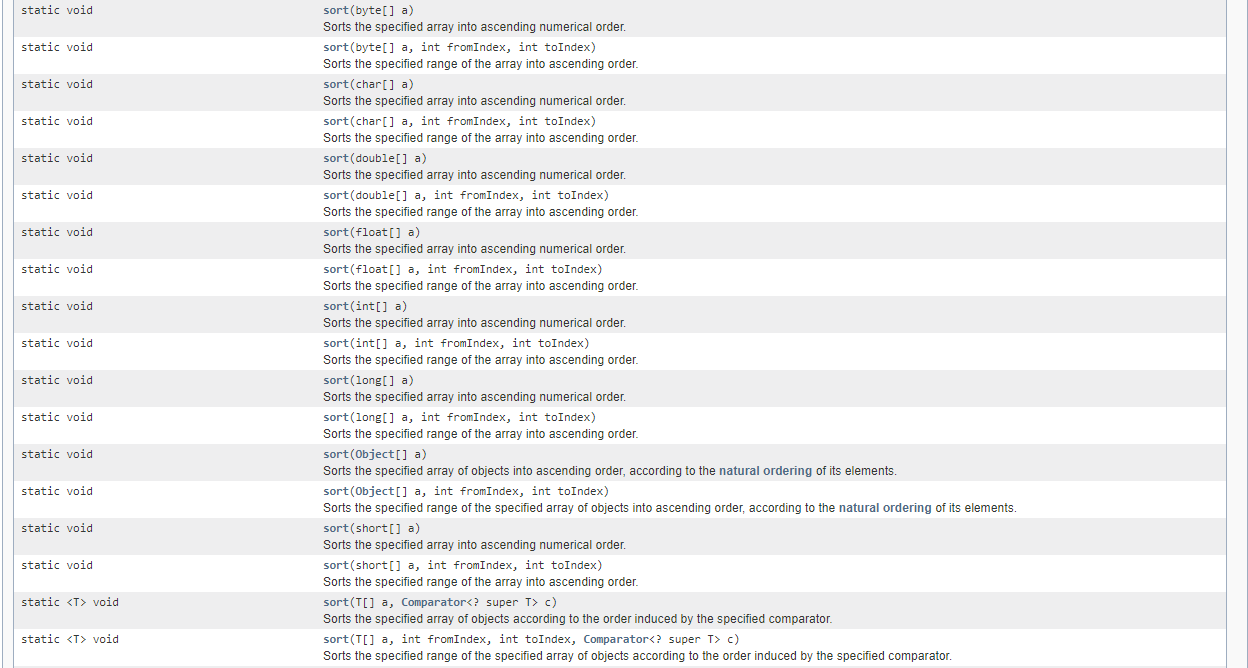
\includegraphics[width=16cm,height=15cm]{Imagen2} 
\vskip 0.4cm
y finalmente el metodo Collections.sort() de Java. Este metodo pertecene a la clase java.Util.Collections. Es usado para ordenar elementos de una lista en orden ascendente. La ventaja con respecto a la anterior es que funciona para colecciones de objetos como por ejemplo ArrayList , LinkedList. El metodo sort sabe perfectamente como ordenar el listado segun los parametros que este posea ya sean string, int, date,etc.
Ahora si queremos que entrege los datos de manera descendente podemos usar el metodo Collections.sort(lista,Collections.reverseOrder()).
\vskip 0.4cm
Por otra parte si tenemos una lista de objetos personalizados (clase estudiante) con variados atributos, para que tenga un orden natural definido, se debe implementar una clase con la interfaz Comparator que hace uso del metodo compare() y a traves de ella determinar por cual atributo sera ordenado. Para que luego se pueda hacer uso del metodo Collections.sort(lista,new OrdenarporID())
\vskip 0.4cm
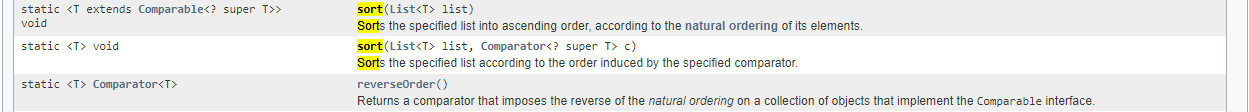
\includegraphics[width=17cm,height=2cm]{Imagen3} 
\vskip 0.4cm
%-------------------------------------------------------------------------
\newpage
\section{Insertion Sort}
\vskip 0.4cm
InsertionSort (ordenamiento por inserción) es la manera natural que el humano ordena, usado comúnmente en el ordenamiento de datos cuantitativos y cualitativos prioritarios.
\vskip 0.4cm
{\bf\underline {Análisis:}}
\vskip 0.4cm
Ordenamiento, que requiere O(n2) operaciones, para cumplir su objetivo en listas o arreglos de n-elementos. Basando en la instrucción básica de:
\begin{itemize}
\item	El tener una lista de j números ordenados, se toma el elemento j+1(el elemento nuevo a insertar).
\item	Se compara iterativamente con los elementos contenidos en la lista si j+1 es menor
\begin{itemize}
\item Si el elemento es menor, el elemento consultado se desplaza a la derecha
\item Si el elemento no es menor se inserta en la posición +1 de la que se consulta (con los mayores desplazados a la derecha si es el caso)
\item Si no se encuentra menor, el elemento j+1 se inserta al principio, dado que el elemento es el menor a los que ya están en la lista desplazados
\end{itemize}
\end{itemize}
\vskip 0.4cm
{\bf\underline {Diseño:}}

\vskip 0.4cm
Con el análisis del funcionamiento del método de ordenamientos por inserción, se diseñó el funcionamiento de la inserción y su ordenamiento. El cual consistió en separar la inserción del ordenamiento principalmente, dado que para este tipo de ordenamiento es válido la inserción de objetos ya sean primitivos o no, de manera individual como en un arreglo y/o lista no ordenado.
\vskip 0.4cm
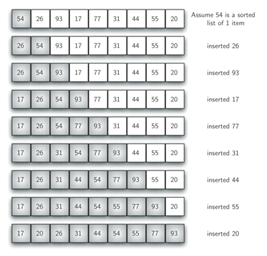
\includegraphics[width=8cm,height=9cm]{Imagen4} 
\vskip 0.4cm
Forma de ordenamiento general en base a comparaciones de cualidades mayores o menores en importancia, siendo en el ordenamiento de números el orden natural de menos a mayor.
\vskip 0.4cm
Orden ejecutado en listas, para su mejor adaptabilidad y uso de recursos.
\vskip 0.4cm
Usando ArrayList $<$E\textgreater y sus métodos de consulta y modificación, además del método compareTo() para comparar cualidades de una clase, definida en Alumno para esta actividad.
\vskip 0.4cm
{\bf\underline {Implementación:}}
\vskip 0.4cm
Luego de conocer el funcionamiento y cualidades que se le otorgaría al algoritmo, se implementó la clase API de “InsertionSort.java”, que contenía en si los métodos de inserción de primitivos enteros “InsertarListaEnteros(ArrayList$<$Enteger\textgreater lista, int valor)”, la cual cumple la función de insertar directamente en la lista entregada para su ordenamiento posterior, llamado dentro del método.
\vskip 0.4cm
Código del método de inserción:
\vskip 0.4cm
\begin{lstlisting}
if(!lista.contains(valor)) {
	lista.add(valor);
}else {
	System.out.print("(el valor existe) ");
}	
if(lista.size() > 1) {
	ordenarListaEnteros(lista);
}
\end{lstlisting}
\vskip 0.4cm
El método de ordenamiento posterior, es de uso público, es decir que su función es para ordenar en la inserción individual de datos, como inserción masiva a través de lista, método llamado “ordenarListaEnteros(ArrayList$<$Integer\textgreater lista)”, que iteraba la lista entregada, comparando y desplazando el contenido en esta para la inserción o remplazo en la posición óptima.
\vskip 0.4cm
Código del método de orden:
\vskip 0.4cm
\begin{lstlisting}
int tam = lista.size();
for(int i = 1;i < tam;i++) {
	int aux = lista.get(i);
	for(int j = i;j > 0;j--) {
		if(aux < lista.get(j-1)) {
			lista.set(j, lista.get(j-1));
			lista.set(j-1,aux);
			imprimirListaEnteros(lista);
		}else {
			break;
		}
	}
}
\end{lstlisting}
\vskip 0.4cm
Y el ultimo método implementado fue la Impresión de datos de la lista, tanto de forma ordenada luego de transcurrido los procesos anteriores de ordenamiento, pero además implementada para la muestra de la condición de la lista mientras se ordenaba iterativamente y mostrar su función de forma visual.
\vskip 0.4cm
Código del método de impresión de enteros:
\vskip 0.4cm
\begin{lstlisting}
Public static void imprimirListaEnteros(ArrayList<Integer> lista) {
	System.out.println(lista);
}
\end{lstlisting}
\vskip 0.4cm
Codigo metodo de impresión de Clase Alumno:
\vskip 0.4cm
\begin{lstlisting}
public static void imprimirListaAlumno(ArrayList<Alumno> lista) {
	int tam = lista.size();
	for(int i = 0;i < tam;i++) {
		System.out.print("  Nombre: "+lista.get(i).getNombre());
		System.out.print("  Apellido: "+lista.get(i).getApellido());
		System.out.print("  Edad: "+lista.get(i).getEdad());
		System.out.println("  Nota: "+lista.get(i).getNota());
	}
}
\end{lstlisting}
\vskip 0.4cm
Estos ordenamientos básicos de enteros, luego fueron usados para los ordenamientos particulares de la clase alumno, con respecto a sus distintas variables, implementando de forma particular cada ordenamiento para su uso único en la opción requerida para ordenar, cualidades como nombre, apellidos, edad y notas, variables de la clase “Alumno.java”.
\vskip 0.4cm
UML
\vskip 0.2cm
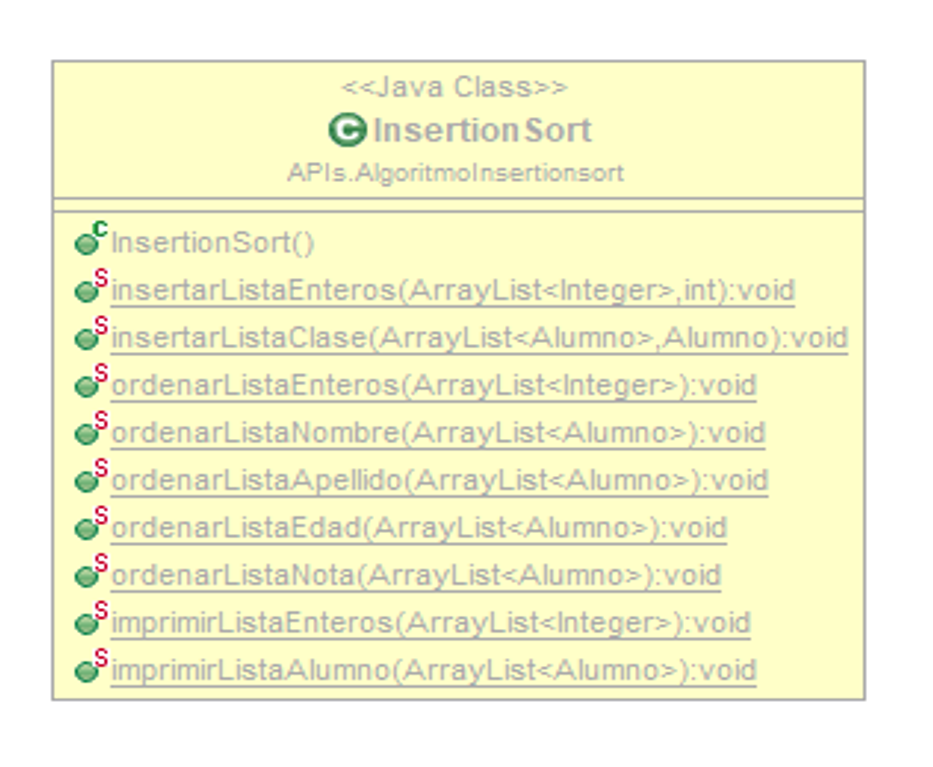
\includegraphics[width=11cm,height=9cm]{Imagen5} 
\vskip 0.4cm
%-------------------------------------------------------------------------
\newpage
\section{Merge sort}
\vskip 0.4cm
Dentro de los métodos de ordenamiento, se encuentran los ordenamientos por comparaciones. Mergesort es uno de ellos y es uno de los más eficaces O(nlogn) lo cual es un costo muy bueno para el tipo de ordenamiento (el mejor caso para los métodos de comparaciones es O(nLogn)).
\vskip 0.4cm
{\bf\underline {Análisis del algoritmo:}} Luego de saber que hace Mergesort, lo siguiente es saber como lo hace y para ello está el siguiente algoritmo:
\vskip 0.4cm
\begin{lstlisting}
MergeSort(arr[], l,  r)
If r > l
     1. Find the middle point to divide the array into two halves:  
             middle m = (l+r)/2
     2. Call mergeSort for first half:   
             Call mergeSort(arr, l, m)
     3. Call mergeSort for second half:
             Call mergeSort(arr, m+1, r)
     4. Merge the two halves sorted in step 2 and 3:
             Call merge(arr, l, m, r)
\end{lstlisting}
\vskip 0.4cm
Como vemos, Mergesort realiza llamadas recursivas para llevar a cabo el método de ordenamiento el cual particiona el arreglo a la mitad recursivamente de izquierda a derecha para luego ordenar los sub arreglos.
\vskip 0.4cm
%-------------------------------------------------------------------------
\newpage
{\bf\underline {Diseño del algoritmo:}}
\vskip 0.4cm
Para el diseño del algoritmo se elaboró el siguiente UML:
\vskip 0.2cm
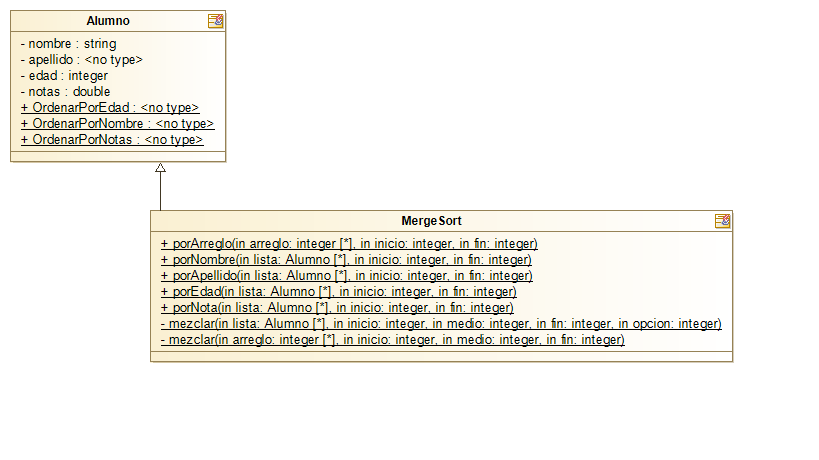
\includegraphics[width=15cm,height=10cm]{Imagen6} 
\vskip 0.4cm
En la cual se utiliza una clase “Alumno” implementada por Gonzalo Villalobos de la cual sus instancias serán ordenadas dentro de una lista de tipo ArrayList. El algoritmo puede ordenar por diferentes criterios (los cuales son los atributos de la clase Alumno) según lo que requiera el jefe de proyecto.
\vskip 0.4cm
%-------------------------------------------------------------------------
\newpage
\section{Quick.sort}
\vskip 0.4cm
En el desarrollo de este software la primera etapa de elaboración se investigo el funcionamiento del algoritmo y se practico de forma manual para comprender de manera correcta y completa.
\vskip 0.4cm
El funcionamiento del algoritmo se puede resumir de la siguiente manera.
\vskip 0.4cm
\begin{itemize}
\item Elegir un elemento de la lista de elementos a ordenar, al que llamaremos pivote.
\item	Resituar los demás elementos de la lista a cada lado del pivote, de manera que a un lado queden todos los menores que él, y al otro los mayores. Los elementos iguales al pivote pueden ser colocados tanto a su derecha como a su izquierda, dependiendo de la implementación deseada. En este momento, el pivote ocupa exactamente el lugar que le corresponderá en la lista ordenada.
\item La lista queda separada en dos sublistas, una formada por los elementos a la izquierda del pivote, y otra por los elementos a su derecha.
\item Repetir este proceso de forma recursiva para cada sublista mientras éstas contengan más de un elemento. Una vez terminado este proceso todos los elementos estarán ordenados.
\end{itemize}
\vskip 0.4cm
La elección del pivote es de suma importancia para la eficiencia del algoritmo, la cual se puede dividir en tres casos:
\vskip 0.4cm
1.	En el mejor caso, el pivote termina en el centro de la lista, dividiéndola en dos sublistas de igual tamaño. En este caso, el orden de complejidad del algoritmo es O(n·log n).
\vskip 0.4cm
2.	En el peor caso, el pivote termina en un extremo de la lista. El orden de complejidad del algoritmo es entonces de O($n^2$). El peor caso dependerá de la implementación del algoritmo, aunque habitualmente ocurre en listas que se encuentran ordenadas, o casi ordenadas. Pero principalmente depende del pivote, si por ejemplo el algoritmo implementado toma como pivote siempre el primer elemento del array, y el array que le pasamos está ordenado, siempre va a generar a su izquierda un array vacío, lo que es ineficiente.
\vskip 0.4cm
3.	En el caso promedio, el orden es O(n·log n).
\vskip 0.4cm
Para la implementación del algoritmo se definió el pivote en la mitad de la lista y así poder obtener una implementación promedio y un costo de O(n·log n). No se definió una forma mas optima en la que se elije el pivote porque se le dio prioridad a la creación del algoritmo para valores primitivos y genéricos.
\vskip 0.4cm
Se desarrollaron dos clases, una clase para primitivos, donde se ordenan valores integer almacenados en un arreglo INT [], y otra clase con valores genéricos donde se recibe un List genérico LIST $<$T\textgreater que se ordenan de igual manera como en los primitivos.
\vskip 0.4cm
Para el diseño del algoritmo se elaboró el siguiente UML:
\vskip 0.2cm
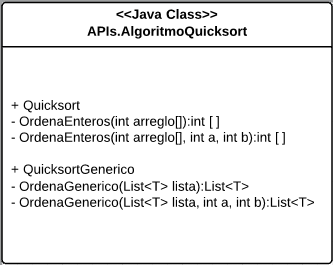
\includegraphics[width=9cm,height=9cm]{Imagen7} 
%-------------------------------------------------------------------------
\newpage
\section{Arrays.sort() y Collections.sort()}
\vskip 0.4cm
{\bf\underline {Análisis:}} La tarea que se me asigno fue ocupar los métodos Arrays.sort() y Collections.sort().
 El primer paso a seguir fue buscar información sobre estos métodos. Ya que en el curso de POO (Programación orientada a objetos) se ven estos métodos en la última parte del curso, sabía como usarlos pero no sabía en detalle el funcionamiento.
 \vskip 0.4cm
Arrays.sort():
\vskip 0.4cm
\begin{itemize}
\item Proviene de la clase Arrays.
\item Ordena el arreglo especificado en orden numérico ascendente.
\item El algoritmo de ordenamiento es un Quicksort Dual-Pívot de Vladimir Yaroslavskiy, Jon Bentley y Joshua Bloch. Este algoritmo ofrece el rendimiento O (n log (n)) en muchos conjuntos de datos que hacen que otras unidades rápidas se degraden a rendimiento cuadrático, y suele ser más rápido que las implementaciones tradicionales (de un solo pivote) Quicksort.
\end{itemize}
\vskip 0.4cm
Collections.sort():
\vskip 0.4cm
\begin{itemize}
\item Proviene de la clase Collections.
\item Este método compara los elementos dentro de una lista antes de ordenar implementando dos interfaces:
\begin{itemize}
\item Comparable: Ordena la lista especificada en orden ascendente, según el orden natural de sus elementos. Todos los elementos en la lista deben implementar la interfaz comparable. Implementa el método compareTo().
\item Comparator: Ordena la lista especificada de acuerdo con el orden inducido por el comparador especificado. Todos los elementos en la lista deben ser mutuamente comparables usando el comparador especificado. Implementa el método compare().
\end{itemize}
\item El algoritmo de ordenamiento es un mergesort estable, adaptable e iterativo que requiere muchas menos comparaciones que n log (n) cuando el conjunto de entrada está parcialmente ordenado, mientras que ofrece el rendimiento de un mergesort tradicional cuando el conjunto de entrada se ordena al azar. Si la lista de entrada está casi ordenada, la implementación requiere aproximadamente n comparaciones. Los requisitos de almacenamiento temporal varían desde una
pequeña constante para listas de entrada casi ordenadas hasta n / 2 referencias de
objetos para listas de entrada ordenadas al azar.
\end{itemize}
{\bf\underline {Diseño:}} Luego de analizar los métodos pasamos a diseñar nuestra API. Para esto se toma
el trabajo realizado en POO en la parte de genéricos del curso.
\vskip 0.4cm
Para ordenar datos primitivos (enteros), creamos una clase llamada OrdenaArreglo la cual
implementa un método que invoca al método arrays.sort.
\vskip 0.4cm
Para ordenar datos no primitivos (basados en clases), creamos una clase llamada Alumno
que contiene 4 atributos: apellido, nombre, edad y nota, la cual nos servirá para crear
objetos de tipo Alumno y se procederá a ordenarlos por los distintos atributos que
contiene la clase. Dentro de esta clase implementamos dos interfaces: comparable y
comparator. La interface comparable implementa el método compareTo que compara en
orden natural. En este caso el orden natural seria ordenar alumnos por su apellido. La
interface comparator implementa el método compare que lo usaremos para comparar por
nombre, por edad y por notas. Luego de esto creamos una clase llamada
OrdenaCollections la cual implementa cuatro métodos para ordenar por apellido, por
nombre, por edad y por nota. Estos 4 métodos invocan el método collections.sort para
ordenar según corresponda.
\vskip 0.4cm

{\bf\underline{Implementación:}} Se procedió a implementar lo descrito en el diseño en la primera
iteración sin mayores inconvenientes. En los métodos que ordenan la clase alumno se
crearon 4 clases aparte de la de alumno para llevar a cabo el ordenamiento. 3 clases que
implementaban la interface comparator con el método compare para comparar por
nombre, edad y nota, y otra que implementaba la los collections.sort según corresponda.
\vskip 0.4cm
En una segunda iteración se cambió esa estructura y los métodos para comparar se fueron
todos a la clase alumno (compara por apellido, por nombre, por edad y por nota). La clase
OrdenaCollection quedo igual con sus métodos que invocan los métodos collections.sort
según corresponda.
\vskip 0.4cm
Para el diseño del algoritmo se elaboró el siguiente UML:
\vskip 0.2cm
\begin{flushright}
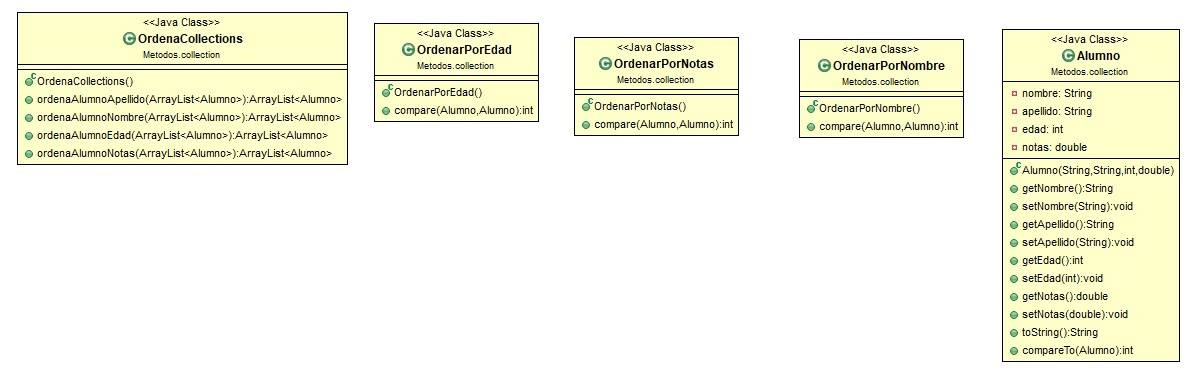
\includegraphics[width=18cm,height=10cm]{Imagen8}
\end{flushright} 
%-------------------------------------------------------------------------
\newpage
\section{Diferencia entre los algoritmos Insertion sort, Merge sort y Quick sort}
\vskip 0.4cm
Los algoritmos se distinguen por las siguientes características:
\vskip 0.4cm
\begin{itemize}
\item Complejidad computacional (peor caso, caso promedio y mejor caso) en términos de n, el tamaño de la lista o arreglo. Para esto se usa el concepto de orden de una función y se usa la notación O(n). El mejor comportamiento para ordenar (si no se aprovecha la estructura de las claves) es O(n log n). Los algoritmos más simples son cuadráticos, es decir O($n^2$). Los algoritmos que aprovechan la estructura de las claves de ordenamiento (p. ej. bucket sort) pueden ordenar en O(kn) donde k es el tamaño del espacio de claves. Como dicho tamaño es conocido a priori, se puede decir que estos algoritmos tienen un desempeño lineal, es decir O(n).
\item Uso de memoria y otros recursos computacionales. También se usa la notación O(n).
\end{itemize}
\vskip 0.2cm

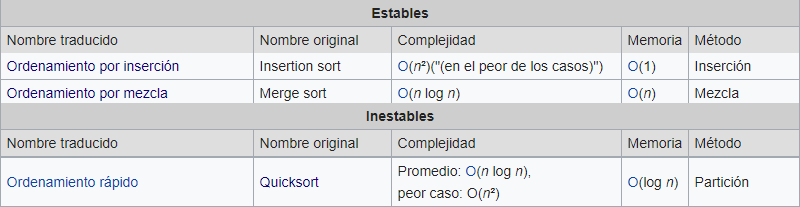
\includegraphics[width=17cm,height=7cm]{Imagen9}

\vskip 0.4cm
%-------------------------------------------------------------------------
\newpage
\section{Diferencias entre Arrays.sort() y Collections.sort() con respecto a los algoritmos de ordenamiento}
\vskip 0.4cm
Arrays.sort() vs Collections.sort()
\vskip 0.4cm
Arrays.sort funciona para matrices que ser de tipo de datos primitivos. En cambio Collections.sort () funciona para colecciones de objetos como ArrayList, LinkedList, etc.

Arrays.sort utiliza el algoritmo de ordenamiento Quicksort Dual-Pivot de Vladimir Yaroslavskiy, Jon Bentley y Joshua Bloch. Este algoritmo ofrece el rendimiento O (n log (n)) en muchos conjuntos de datos que hacen que otras unidades rápidas se degraden a rendimiento cuadrático, y suele ser más rápido que las implementaciones tradicionales (de un solo pivote) Quicksort.

Collection.sort implementa un mergesort estable, adaptable e iterativo que requiere muchas menos comparaciones n log (n) cuando el conjunto de entrada está parcialmente ordenado, mientras que ofrece el rendimiento de un mergesort tradicional cuando el conjunto de entrada se ordena al azar. Si la matriz de entrada está casi ordenada, la implementación requiere aproximadamente n comparaciones.
%-------------------------------------------------------------------------
\newpage
\vskip 0.4cm
\section{Conclusión}
\vskip 0.4cm
A través del trabajo de los distintos métodos de ordenamiento, junto a el análisis de los algoritmos a trabajar, existió libertad de manejo de estos, a través de las diversas herramientas de java. Aunque existiera simplicidad en la forma que se ven los ordenamientos en la vida cotidiana, estos conllevan instrucciones específicas que no siempre manejamos, y solo realizamos el orden sin conocer todo el proceso de las decisiones que ocurren en el trasfondo. En este trabajo, e investigación, se muestra como vemos de forma natural los ordenamientos, transcrito a órdenes para la automatización de las decisiones, que llevan a un resultado óptimo para su manejo, e interpretación. Los algoritmos vistos, fueron la manera de relacionar las diversas formas de orden, aunque limitado a lo investigado, y lo implementado, con cosas simples y rutinarias. El trabajo se desarrolló en armonía con el grupo de trabajo, con las instrucciones a tiempo, para lograr un análisis, diseño e implementación requeridos en la funcionabilidad final, junto a las adiciones necesarias para que el trabajo no solo cumpla, sino también represente el esfuerzo, compromiso y motivación en nuestro trabajo final que será por largo tiempo el programar, tanto ideas como soluciones a través de la computación. 
\vskip 0.4cm
\newpage
\begin{thebibliography}{10}
\bibitem{}{Algoritmos de Ordenamiento: monografias.com/trabajos/algordenam/algordenam.shtml}
\bibitem{}{Algoritmos de Ordenamiento: lwh.free.fr/pages/algo/tri/tri\_es.htm}
\bibitem{}{Algoritmos de Ordenamiento: es.wikipedia.org/wiki/Algoritmo\_de\_ordenamiento}
\bibitem{}{Algoritmo Insertion Sort: en.wikipedia.org/wiki/Insertion\_sort}
\bibitem{}{Algoritmo Merge Sort: en.wikipedia.org/wiki/Merge\_sort}
\bibitem{}{Algoritmo Quick Sort: es.wikipedia.org/wiki/Quicksort}
\bibitem{}{Algoritmo Quick Sort: geeksforgeeks.org/quick\-sort}
\bibitem{}{Documentación Collections.Sorts: docs.oracle.com/javase/7/docs/api/java/util/Collections.html}
\bibitem{}{Metodo Collections.sort(): stackoverflow.com/questions/6957631/sort\-java\-collection}
\bibitem{}{Ejemplos Arrays.sort(): geeksforgeeks.org/arrays\-sort\-in\-java\-with\-examples}
\bibitem{}{Ejemplos Collections.sort(): geeksforgeeks.org/collections\-sort\-java\-examples}
\bibitem{}{Ejemplos Comparator: journaldev.com/780/comparable\-and\-comparator\-in\-java-example}
\bibitem{}{Ejemplos Comparable y Comparator: mkyong.com/java/java\-object\-sorting\-example\-comparable\-and\-comparator}
\bibitem{}{Introduction to Algorithms CLRS}
\bibitem{}{[Cormen-AL2011]Introduction\_To\_Algorithms-A3}
\end{thebibliography}
\end{document}